\section{Άσκηση 3}
\subsection{Θεωρητική Ανάλυση}
Αυτήν την φορά, αντί να χρησιμοποιήσουμε γραμμική ανάδραση καταστάσεων, θα αξιοποιήσουμε δυναμική ανάδραση καταστάσεων, για να επιτύχουμε απόσβεση των διαταραχών (δηλαδή του μαγνητικού φρένου) και σύγκλιση της θέσης του κινητήρα στην επιθυμητή τιμή. Γι'αυτό, ορίζουμε μια νέα μεταβλητη κατάστασης $z$, τέτοια ώστε $\dot{z} = y - r = x_2 - r$. Έτσι, το σύστημα γίνεται
\begin{align*}
	\dot{x} &= Ax + Bu \\
	\dot{z} &= y - r
\end{align*}
Δηλαδή, η τάξη του συστήματος αυξήθηκε. Στη σημείο ισορροπίας εξ' ορισμού θα ισχύει $\dot{x} = 0$ και \\$\dot{z} = 0 \Rightarrow y = x_2 = r$, οπότε θα έχουμε φτάσει στο θεμιτό αποτέλεσμα. Άρα, αρκεί να φροντίσουμε το συστημα να είναι ασυμπτωτικά ευσταθές, διότι έτσι σίγουρα θα συγκλίνουμε στο σημείο ισορροπίας. 

Ορίζουμε, λοιπόν, ελεγκτή $u=-\tilde{k}\tilde{x}$, όπου $\tilde{k} = \begin{bmatrix} k & k_i \end{bmatrix}$ και $\tilde{x} = \begin{bmatrix} x \\ z \end{bmatrix}$. Ο όρος $k_rr$ που είχαμε στην προηγούμενη άσκηση δεν χρειάζεται πλέον, αφού όπως είπαμε η έξοδος με τον τωρινό ελεγκτή θα είναι συγκεκριμένη. Επομένως, $u=-kx-k_iz$ και το σύστημα γίνεται
\begin{align*}
    \begin{bmatrix} 
        \dot{x}_1 \\ \dot{x}_2 \\ \dot{z} 
    \end{bmatrix} 
    &= 
    \begin{bmatrix}
        -\frac{1}{T_m} & 0 & 0 \\
        k_μk_0 & 0 & 0 \\ 
        0 & 1 & 0 
    \end{bmatrix}
    \begin{bmatrix}
        x_1 \\
        x_2 \\
        z
    \end{bmatrix} + 
    \begin{bmatrix}
        \frac{k_m}{T_m} \\
        0 \\ 
        0
    \end{bmatrix} u + 
    \begin{bmatrix}
        0 \\
        0 \\
        -1
    \end{bmatrix} r \\
    &=
    \begin{bmatrix}
        -\frac{1}{T_m} & 0 & 0 \\
        k_μk_0 & 0 & 0 \\ 
        0 & 1 & 0 
    \end{bmatrix}
    \begin{bmatrix}
        x_1 \\
        x_2 \\
        z
    \end{bmatrix} + 
    \begin{bmatrix}
        \frac{k_m}{T_m} \\
        0 \\ 
        0
    \end{bmatrix} (-k_1x_1 -k_2x_2 - k_iz) +
    \begin{bmatrix}
        0 \\
        0 \\
        -1
    \end{bmatrix} r \\
    &=
    \underbrace{
    \begin{bmatrix}
        -\frac{1+k_mk_1}{T_m} & -\frac{k_2}{T_m} & -\frac{k_i}{T_m} \\
        k_μk_0 & 0 & 0\\
        0 & 1 & 0
    \end{bmatrix}}_{\tilde{A}}
    \begin{bmatrix}
        x_1 \\
        x_2 \\
        z
    \end{bmatrix} + 
    \begin{bmatrix}
        0 \\
        0 \\
        -1
    \end{bmatrix} r
\end{align*}
Με χαρακτηριστικό πολυώνυμο
\[
	P(s) = det(sI - \tilde{A}) = s^3 + \frac{1+k_mk_1}{T_m}s^2 + \frac{k_μk_0k_mk_2}{T_m}s + \frac{k_μk_0k_mk_i}{T_m}
\]
Θέλουμε το σύστημα να είναι ευσταθές, άρα απο κριτήριο Routh-Hurwitz πρέπει
\[
\renewcommand{\arraystretch}{2.5}
\left.
\begin{array}{l}
	\frac{1 + k_m k_1}{T_m} > 0 \\ 
	\frac{k_μk_0k_mk_2}{T_m} - \frac{k_μk_0k_mk_i}{1+k_mk_1} > 0\\
    \frac{k_μk_0k_mk_i}{T_m} > 0
\end{array}
\right\}
\Rightarrow
\left.
\begin{array}{l}
	k_1 > -\frac{1}{k_m} = -\frac{1}{218.89} = -4.57 \cdot 10^{-3} \\
	k_i < \frac{k_2(1+k_mk_1)}{T_m} \\
    k_i > 0
\end{array}
\right\}
\renewcommand{\arraystretch}{1}
\]
\subsection{Εργαστηριακά Αποτελέσματα}
Έπειτα από αρκετές δοκιμές για την επιλογή των κατάλληλων κερδών, καταλήξαμε στις τιμές \\$k_1 = 0.01,\ k_2 = 6,\ k_i = 5$, οι οποίες ικανοποιούν τους πιο πάνω περιορισμούς. Αυτές μας δίνουν τα παρακάτω αποτελέσματα. Παρατηρούμε ότι αν και ο χρόνος αποκατάστασης είναι πιο αργός από όταν χρησιμοποιήσαμε γραμμική ανάδραση καταστάσεων, το σφάλμα θέσης στην μόνιμη κατάσταση πλέον είναι μηδενικό. Αυτό δεν συνέβαινε προηγουμένως. Φυσικά, και εδώ φροντίσαμε ώστε να μην έχουμε υπερύψωση.
\begin{figure}[H]
    \centering
    \begin{minipage}{0.45\textwidth}
        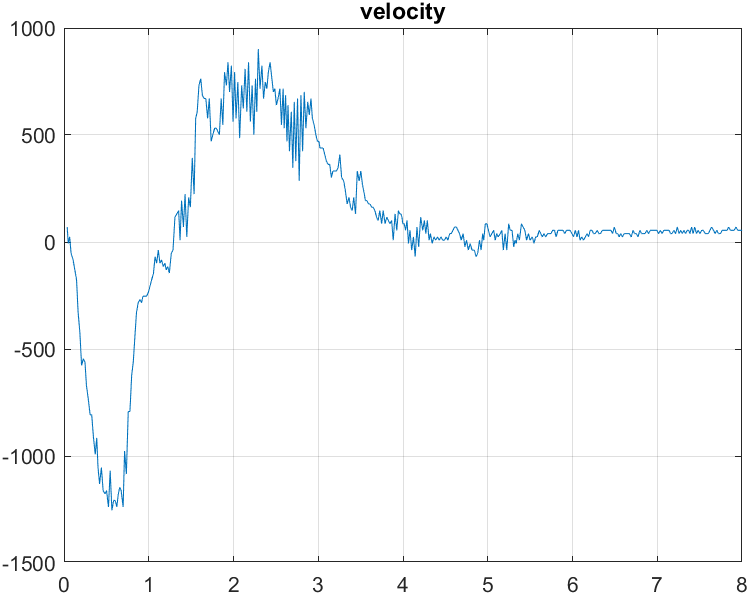
\includegraphics[width=\linewidth]{Images/lab3/vel32.png}
    \end{minipage}
    \hfill
    \begin{minipage}{0.45\textwidth}
        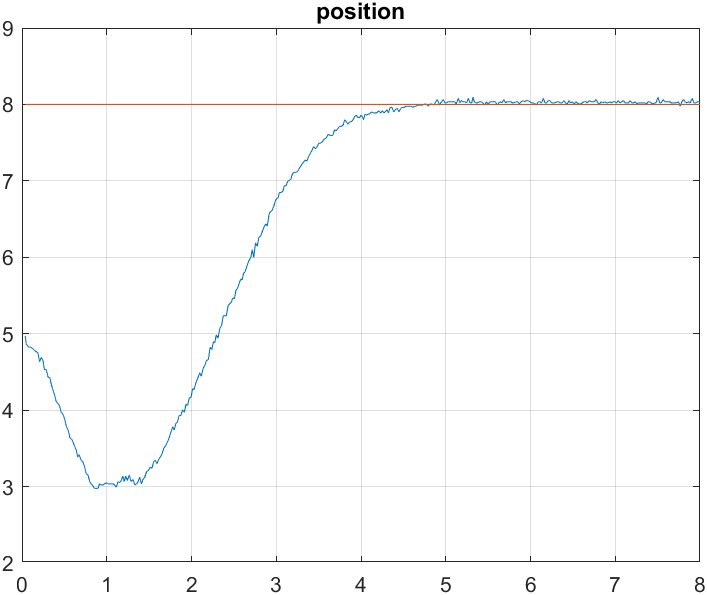
\includegraphics[width=\linewidth]{Images/lab3/pos32.png}
    \end{minipage}
    \end{figure}
    \begin{figure}[H]
    \begin{minipage}{0.45\textwidth}
        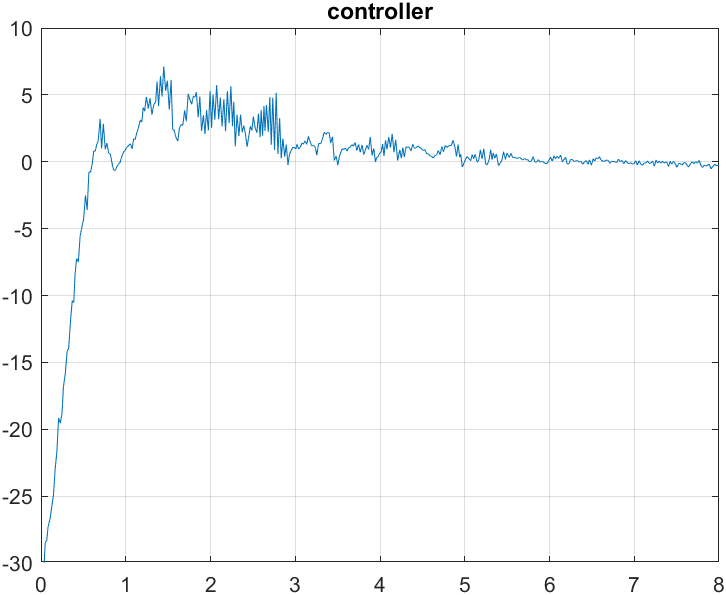
\includegraphics[width=\linewidth]{Images/lab3/con32.png}
    \end{minipage}
    \hfill
    \begin{minipage}{0.45\textwidth}
        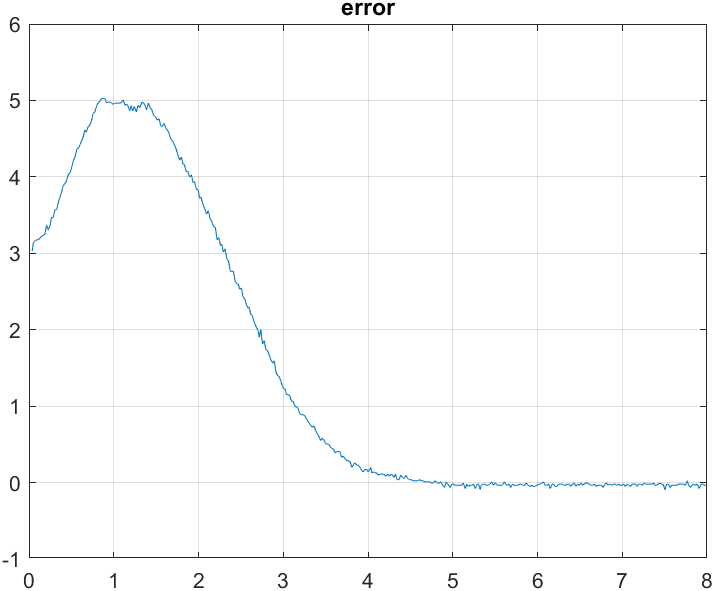
\includegraphics[width=\linewidth]{Images/lab3/err32.png}
    \end{minipage}
\end{figure}
\begin{figure}[H]
    \centering
    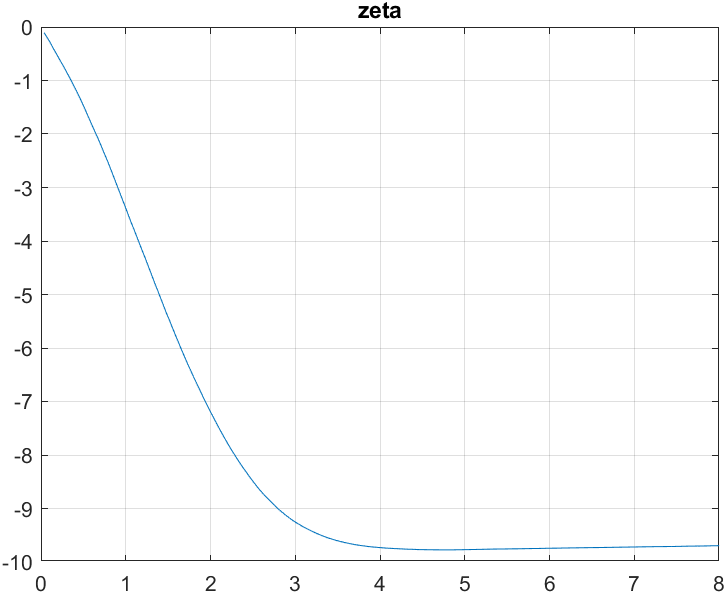
\includegraphics[width=0.5\linewidth]{Images/lab3/zet32.png}
\end{figure}
